\documentclass[11pt]{report}

\usepackage[left=0.75in, right=0.75in, top=0.75in, bottom=0.75in]{geometry}
\usepackage{layout}
\usepackage{ucs}
\usepackage[utf8x]{inputenc}
\usepackage{titlesec}
\usepackage{graphicx}
\usepackage{amssymb}
\usepackage{amsmath}
\usepackage{dsfont}
\usepackage{float}
\usepackage{caption}
\usepackage{subcaption}
\usepackage{array}



\title{\textbf{TS114 Project}\\Computer-aided analysis of electrocardiogram signals}
\author{{Maxime PETERLIN - Gabriel VERMEULEN }\\\\{ENSEIRB-MATMECA, Bordeaux}}
\date{June, 6th 2014}


\begin{document}


\maketitle

\tableofcontents

\newpage
\section*{Introduction}


\chapter{ECG visualization}
	In this first part, seven different ECG signals will be analyzed and displayed under MATLAB. \\Three of these are records from healthy patient's heart, whereas the other four are from ill ones, each with different pathologies.\\
	This part's aim is to study these signals in the frequency and time domain, starting by the latter, and underline the different caracteristics and properties of these.

	\section{Time display}
		\begin{figure}[ht]
			\centering
			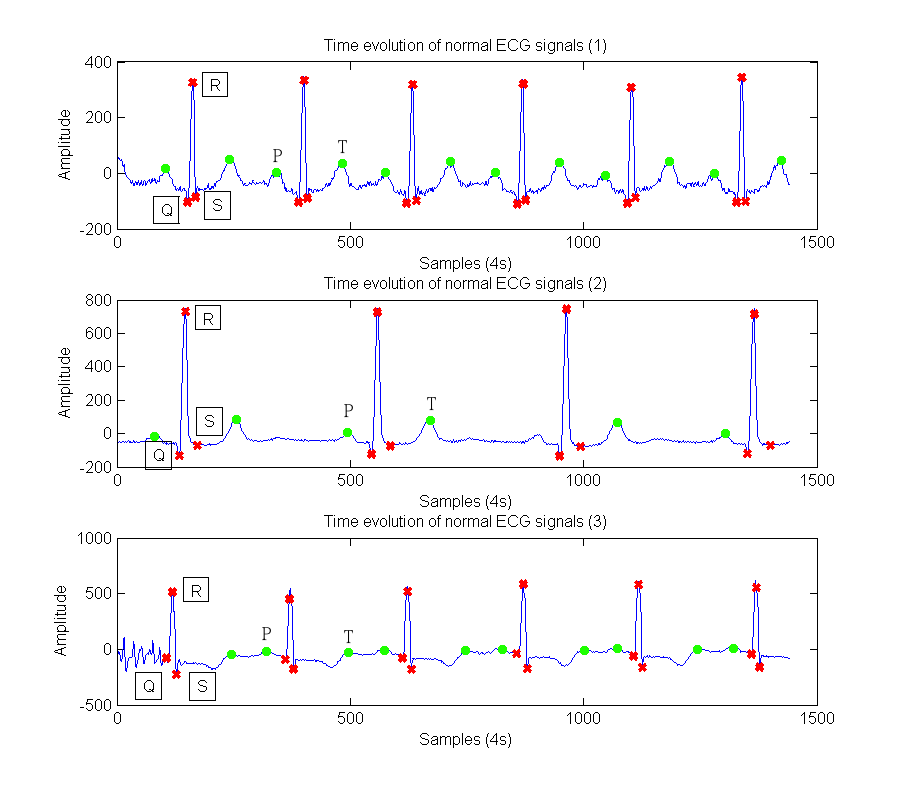
\includegraphics[scale=0.65]{images/Q311_1.png}
			\caption{Normal ECG signals with the Q, R, S points and P, T waves highlighted}
			\label{Q311_1}
		\end{figure}

		First, three seconds of each of the aforementioned normal ECG signals (i.e. from healthy heart) were plotted under MATLAB. On the figure above (Figure~\ref{Q311_1}), their Q, R and S points are represented by red dots, while their P and T waves are located by green dots.  \\
		\\
		The first signal displayed is noisier than the two others, although, its characteristic points and waves are easier to observe.\\
		The second signal is uncluttered, but the S point is hardly recognizable.\\
		Finally, the P and T waves of the third signal, which is a tad noisy, are nearly overlapping.\\
		\\
		Based on these four seconds samples, the cardiac rhythm of each patients was computed and displayed in the table below.\\
		\begin{center}
			\begin{tabular}{|c|c|c|}
				\hline
				\textbf{Signal number} & \textbf{Cardiac rhythm (bpm)} \\
				\hline
				1 & 91.7 \\ 
				\hline
				2 & 53.0 \\
				\hline
				3 & 86.4 \\
				\hline
			\end{tabular}
		\end{center}
		According to the graphs and the computed cardiac rhythms, it can be assumed that the faster the heartbeat is, the noiser the ECG will be. Indeed, the first signal is the fastest heartbeat's ECG while being the noisest. The same can be said of the third signal.\\
		Moreover, the second signal represents the ECG of a heart with a slow heartbeat and since it is a normal ECG, it might be the heartbeat of an athletic person (otherwise it coud be a heart condition like bradycardia).\\
		\\
		\begin{figure}[ht]
			\centering
			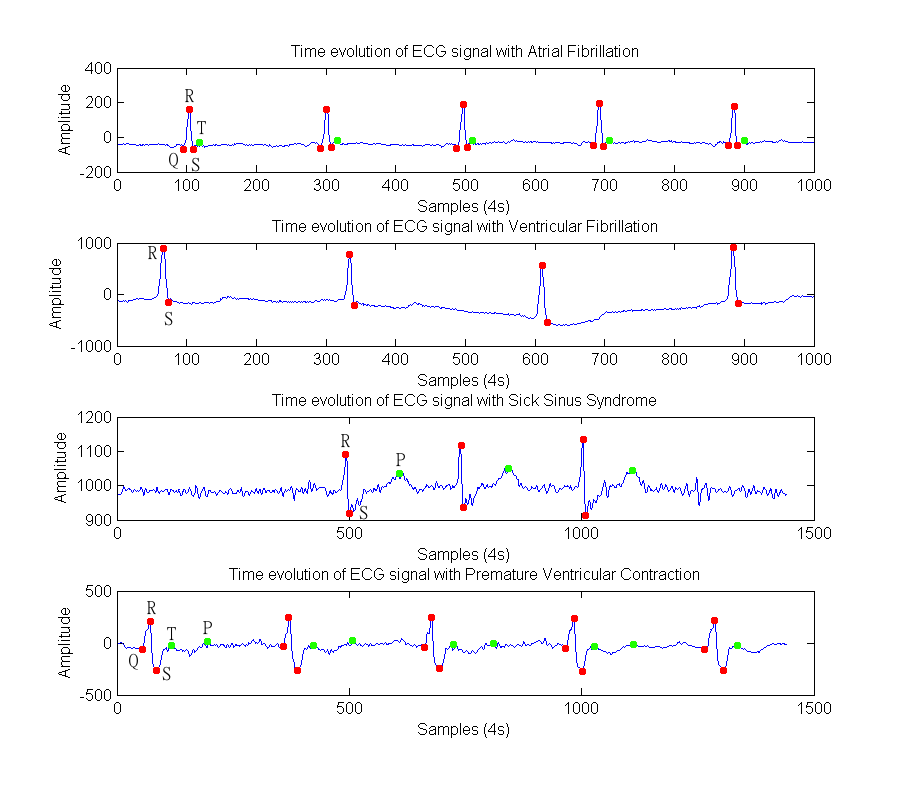
\includegraphics[scale=0.65]{images/Q312_2.png}
			\caption{Normal ECG signals with the Q, R, S points and P, T waves highlighted}
			\label{Q312_2}
		\end{figure}
		\\
		Then, the last four ECG signals associated with heart conditions were plotted under MATLAB.
		\\


	\section{Frequency display}


\chapter{Detection of P, QRS and T waves}

\chapter{Automatic identification of cardiac pathologies}

\chapter{ECG denoising}


\newpage
\section*{Conclusion}

\end{document}
